\documentclass[aspectratio=169]{beamer}

% SETUP =====================================
\usepackage[T1,T2A]{fontenc}
\usepackage[utf8]{inputenc}
\usepackage[russian]{babel}
\usepackage{listings}
\usepackage{amssymb}
\usepackage{minted}
\usepackage{../../beamerthemeslidesgeneric}
% SETUP =====================================

\title{Concurrency in Scala}
\author{Mikhail Mutcianko, Alexey Shcherbakov}
\institute{СПБгУ, СП}
\date{8 апреля 2021}

\begin{document}

\frame{\titlepage}

\section{Concurrent, Parallel, Asynchronous}
% parallel vs concurrent vs asynchronous
\begin{frame}{Concurrent vs Parallel computations}
  \begin{block}{Concurrent}
   Concurrent computing is a form of computing in which several computations are executed
   during overlapping time periods — instead of sequentially, with one completing before
   the next.
  \end{block}

  \begin{block}{Parallel}
    Parallel computations must also advance simultaneously
  \end{block}
\end{frame}

\begin{frame}{Concurrent vs Parallel computations}
  \centering
  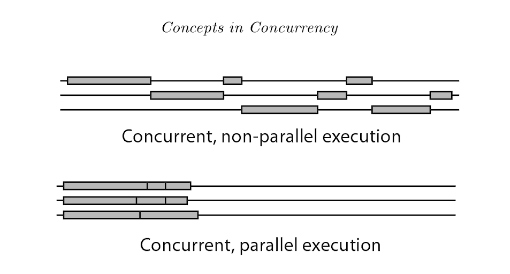
\includegraphics[scale=0.55]{cvp.jpg}
\end{frame}

% synchronous execution
\begin{frame}[fragile]{Synchronous execution}
  \begin{block}{}
    In synchronous model of execution for any statement S of a linear top-down
    program flow, computation of all statements that are defined before S must
    finish by the time S is started.
  \end{block}
  \bigskip
  \pause
  \begin{minted}{scala}
  val a = longComputeA()
  val b = longComputeB() // a is initialized

  longComputeAB(a,b) // both a and b are computed
  \end{minted}
\end{frame}


% scala asynchronous execution
\begin{frame}{Asynchronous execution}
  \begin{block}{}
    Asynchronous computations drop the <<happens before>> requirement.
    Async model allows to continue the next statement even if the previous has not finished yet.
  \end{block}
\end{frame}

\begin{frame}[fragile]{Asynchronous execution}
  \begin{minted}{scala}
  println("starting A")
  val a = Future { longComputeA(); println("A finished") }
  println("starting B")
  val b = Future { longComputeB(); println("B finished") }
  println("starting AB")
  longComputeAB(a,b)
  \end{minted}
  \bigskip
  \pause
  \begin{Verbatim}[fontsize=\tiny,frame=single]
  starting A
  starting B
  starting AB
  A finished
  B finished
  \end{Verbatim}
\end{frame}

\section{Concurrency Primitives}

% runnable and callable
\begin{frame}[fragile]{Runnable and Callable}
  Low-level computation abstractions are defined as traits
  \bigskip
  \begin{minted}{scala}
  // computation does NOT return a value
  trait Runnable {
    def run(): Unit
  }

  // computation returns a value
  trait Callable[V] {
    def call(): V
  }
  \end{minted}
\end{frame}

\begin{frame}[fragile,t]{Thread}
  Scala concurrency is built on top of the Java concurrency model.

  A Thread takes a Runnable. You have to call start on a Thread in order for it to run the Runnable.
\bigskip
\begin{onlyenv}<1>
    \begin{minted}{scala}
  val hello = new Thread(new Runnable {
    def run() {
      println("hello world")
    }
  })
  
  hello.start
  // -> hello world
    \end{minted}
\end{onlyenv}
\begin{onlyenv}<2>
    \begin{minted}{scala}
  val hello = new Thread(() => println("hello world"))

  hello.start
  // -> hello world
    \end{minted}
\end{onlyenv}
\end{frame}

% futures
\section{Futures}
\begin{frame}{Scala Future}
  \begin{block}{}
    Future is an abstraction capturing a computation process
  \end{block}
  \bigskip
  A computation can be in one of the following \textbf{three} states:
  \begin{itemize}
    \item unfinished
    \item successful
    \item failed
  \end{itemize}
\end{frame}

\begin{frame}[fragile]{Future Methods}{Common}
  \mint[linenos=false]{scala}{def Future.apply(f: =>A)|\only<3>{(implicit ec: ExecutionContext)}|: Future[A]}
  \begin{itemize}
    \item accepts a code block
    \item starts computation eagerly
  \end{itemize}
  \bigskip
  \pause
  \mint[linenos=false]{scala}{def onComplete(cb: Try[A] =>B)|\only<3>{(implicit ec: ExecutionContext)}|: Unit}
  \begin{itemize}
    \item provides a callback for a finished computation
  \end{itemize}
\end{frame}

\begin{frame}[fragile]{ExecutionContext}
\begin{block}{}
  An \textit{ExecutionContext} is an abstraction which implementations must provide a concrete mechanism
  of executing computations represented by Scala's \texttt{Future}. The intent of ExecutionContext
  is to lexically scope code execution
\end{block}
\medskip
\begin{itemize}
  \item built-in implementation:\\
    \mintinline{scala}{scala.concurrent.ExecutionContext.Implicits.global}
  \item based on Java's \texttt{ForkJoinPool}
  \item automatically scales to the number of CPU cores
\end{itemize}
\end{frame}

\begin{frame}{Working with results}
  There are several ways of processing an async computation's result:
  \begin{itemize}
    \item block current thread and get a result
    \item execute a callback when a computation finishes
    \item compose another computation
  \end{itemize}
\end{frame}

\begin{frame}{Blocking the result}
An asynchronous computation can be turned into a synchronous one by 
using \texttt{Await.result}
\medskip
\\This method will block the current thread until:
\begin{itemize}
  \item the Future completes(successfully or not)
  \item a timeout occurs
\end{itemize}
\end{frame}

\begin{frame}[fragile]{Blocking the result}{Example}
\begin{minted}{scala}
val greetingFuture = Future {
  Thread.sleep(1000) 
  "Hello" 
}

val greeting: String = Await.result(greetingFuture, Duration.Inf)

println(s"Result: $greeting")
\end{minted}
\end{frame}

\begin{frame}{Blocking the result}{Poor practice}
  \begin{block}{}
    Blocking on a future is strongly discouraged for the sake of performance and for the prevention of
    deadlocks. Callbacks and combinators on futures are a preferred way to use their results.
  \end{block}
\end{frame}

\begin{frame}[fragile]{Blocking the result}{Deadlock example}
\begin{minted}{scala}
implicit val ec = ExecutionContext
  .fromExecutor(Executors.newFixedThreadPool(1))

def addOne(x: Int) = Future(x + 1)

def multiply(x: Int, y: Int) = Future {
  val a = addOne(x)
  val b = addOne(y)
  val result = for (r1 <- a; r2 <- b) yield r1 * r2

  // this will dead-lock
  Await.result(result, Duration.Inf)
}
\end{minted}
\end{frame}

\begin{frame}[fragile]{Using callbacks}{onComplete}
  Processing the result of a Future can be done in a completely non-blocking way by providing a
  callback using: \mintinline{scala}{Future.onComplete[U](f: (Try[T]) => U): Unit}
  \bigskip
  \begin{minted}{scala}
  val f: Future[List[String]] = Future {
    session.getRecentPosts
  }

  f onComplete {
    case Success(posts) => for (post <- posts) println(post)
    case Failure(t) => println("An error has occurred: " + t.getMessage)
  }
  \end{minted}
\end{frame}

\begin{frame}[fragile]{Using callbacks}{foreach}
In the case where only successful results need to be handled, the \texttt{foreach} callback can be used:
\bigskip
\begin{minted}{scala}
val f: Future[List[String]] = Future {
  session.getRecentPosts
}

f foreach { posts =>
  for (post <- posts) println(post)
}
\end{minted}
\end{frame}

\begin{frame}{Callback hell}
  Chaining computations using callbacks is achieved by nesting creation of \texttt{Future}s.\\
  This can lead to severe cases of LOP - Ladder Oriented Programming also known as <<callback hell>>\\
\end{frame}

\begin{frame}[fragile]{Callback hell}{Example}
\begin{minted}{scala}
queryDb(8612).onComplete {
  case Failure(ex: Exception) => 
    println(s"Operation failed with $ex")
  case Success(fileName: String) => 
    loadFileAsync(fileName).onComplete {
      case Failure(ex: Exception) => 
        println(s"Operation failed with $ex")
      case Success(url: String) => 
        loadPageAsync(url).onComplete {
          case Failure(ex: Exception) => println(s"Operation failed with $ex")
          case Success(text: String) => Future { ... }
      ...
}
\end{minted}
\end{frame}

% composing futures
\begin{frame}{Functional composition of Futures}{Monad}
  In Scala a \mintinline{scala}{Future[+A]} is a monad, providing the following methods:
  \begin{itemize}
    \item \mintinline{scala}{def map[B](f: A => B): Future[B]}
    \item \mintinline{scala}{def flatMap[B](f: A => Future[B]): Future[B]}
    \item \mintinline{scala}{def withFilter(f: A => Boolean): Future[A]}
  \end{itemize}
\end{frame}


\begin{frame}[fragile]{Functional composition of Futures}{Example}
Monadic composition style:
\begin{minted}{scala}
  queryDb(8612)
   .flatMap(fileName  => loadFileAsync(fileName))
   .flatMap(url       => loadPageAsync(url))
   .flatMap(pageText  => println(pageText))
\end{minted}
\pause
\bigskip
For-comprehension style:
\begin{minted}{scala}
for {
  fileName  <- queryDb(8612)
  url       <- loadFileAsync(fileName)
  pageText  <- loadPageAsync(url)
} println(pageText)
\end{minted}
\end{frame}

\begin{frame}{Error handling}
  \begin{itemize}
    \item \mintinline{scala}{def recover[U >: T](pf: PartialFunction[Throwable, U]): Future[U]}\\
      \footnotesize Creates a new future that will handle any matching throwable that this future might contain.
    \item \mintinline{scala}{def recoverWith[U >: T](pf: PartialFunction[Throwable, Future[U]]): Future[U]}\\
      \footnotesize Same as \texttt{recover}, but composes another future instead of a value
    \item \mintinline{scala}{def fallbackTo[U >: T](that: Future[U]): Future[U]}\\
      \footnotesize Creates a new future which holds the result of this future if it was completed
      successfully, or, if not, the result of the that future if that is completed successfully.
    \item \mintinline{scala}{def failed: Future[Throwable]}\\
      \footnotesize Returns a Future with an exception as a result value if the original one has
      failed
  \end{itemize}
\end{frame}

\begin{frame}[fragile]{Error handling}{Example}
\begin{minted}{scala}
Future (6 / 0) recover { case e: ArithmeticException => 0 } // result: 0

val f = Future { Int.MaxValue }
Future (6 / 0) recoverWith { case e: ArithmeticException => f } // result: Int.MaxValue

val f = Future { throw new RuntimeException("failed") }
val g = Future { 5 }
val h = f fallbackTo g
h foreach println // Eventually prints 5

val g = Future { 2 / 0 }
for (exc <- g.failed) println(exc) // result: java.lang.ArithmeticException: / by zero
\end{minted}
\end{frame}

\begin{frame}{Future aggregation}
\begin{itemize}
  \item \mintinline{scala}{def traverse(in: M[A])(fn: (A) => Future[B]): Future[M[B]]}\\
    \footnotesize Asynchronously and non-blockingly transforms a \texttt{IterableOnce[A]} into a
    \texttt{Future[IterableOnce[B]]} using the provided function \texttt{A => Future[B]}
  \item \mintinline{scala}{def sequence(in: M[Future[B]]): Future[M[B]]}\\
    \footnotesize Transforms a sequence of futures into a future of sequences
  \item \mintinline{scala}{def zip(other: Future[B]): Future[(A, B)]}\\
    \footnotesize Creates a single future of Tuple2 from two futures
  \item \mintinline{scala}{def foldLeft(futures: Iterable[Future[T]])(zero: R)(op: (R, T) => R): Future[R]}
  \item \mintinline{scala}{def reduceLeft(futures: Iterable[Future[T]])(op: (R, T) => R): Future[R]}
\end{itemize}
\end{frame}

\begin{frame}{Promise}
  \begin{block}{}
    Promise is an API for creating Futures with a controllable state. Promises \textit{complete} the
    Futures they produce(by ''completing`` the promise)
  \end{block}
  The generated Furture state can be controlled with the following:
  \begin{itemize}
    \item \texttt{complete / completeWith}
    \item \texttt{tryComplete / tryCompleteWith}
    \item \texttt{success / trySuccess / failure / tryFailure}
  \end{itemize}
\end{frame}

\begin{frame}[fragile]{Promise}{Example}
\begin{minted}{scala}
val p = Promise[T]()
val f = p.future

val producer = Future {
  val r = produceSomething()
  p success r
  continueDoingSomethingUnrelated()
}

val consumer = Future {
  startDoingSomething()
  f foreach { r => doSomethingWithResult() }
}
\end{minted}
\end{frame}

\begin{frame}{Promise assignment semantics}
      \begin{block}{}
        Promises have single-assignment semantics. As such, they can be completed only once. 
      \end{block}
      \bigskip
      Calling success on a promise that has already been completed (or failed) will throw an
      IllegalStateException
\end{frame}
% TODO: async\await


\section{Parallel Collections}

% scala parallel collections
\begin{frame}[fragile]{Scala parallel collections}
  Scala provides an easy way of converting any sequential collection to parallel with \texttt{.par}
  \bigskip
  \pause
  \begin{minted}{scala}
  val list = (1 to 10000).toList
  list.par.map(_ + 42)
  \end{minted}
  \bigskip
  “out-of-order” semantics of parallel collections lead to the following two implications:
  \begin{itemize}
    \item Side-effecting operations can lead to non-determinism
    \item Non-associative operations lead to non-determinism
  \end{itemize}
\end{frame}

 % TODO: futures as parallel data processors

% TODO: other concurrency models
 % actors - Akka
 % reactive streams - Monix
 % kotlin coroutines vs scala futures
\section{Practice}
\end{document}

